\documentclass[transmag]{IEEEtran}
\usepackage{latexsym}
\usepackage{graphicx}
\usepackage{amsfonts,amssymb,amsmath}
\usepackage{hyperref}

\markboth{$>$ G00359016 $<$}
{$>$ G00359016 $<$}
\begin{document}

\title{Blockchain in IoT: A review of benefits and challenges.}

\author{Anton Golubev}

\IEEEtitleabstractindextext{\begin{abstract}IoT has the potential to transform the world by making everything interconnected through small devices that are connected to one massive network. However, it has some problems such as scalability, cost and security that will need to be resolved before it achieves this goal. Blockchain could potentially be the silver bullet needed to fix these issues. In this article, we review the problems with IoT and how blockchain technology could potentially solve them.\end{abstract}}

\maketitle

\section{INTRODUCTION}

\IEEEPARstart{T}{he} Internet of Things (IoT) is a new technological paradigm. It attempts to connect every device to the internet in real time by connecting a giant global network of smart devices that are capable of interacting with one another. Examples of smart devices include smart phones, tablets, smart cars, smart watches and even smart fridges. Anything that has some kind of sensor would be considered an IoT device. It is a revolutionary technology because the potential benefits to it are vast. It has the potential to improve quality of life in many ways - one example is smart traffic lights, where there are cameras pointed at each road of an intersection and the based on the input of the camera, a program decides when to make the lights green in order to eliminate the wait time that usually happens at a traffic light. The authors of \cite{ref1} identify the two main existing applications of IoT, which are: (i) RFID technology that allows the tracking of anything attached with an RFID tag, and; (ii) Wireless Sensor Networks (WSNs) which measure environmental conditions such as pollution levels, humidity, temperature, wind etc. These could be used in any industry that needs monitoring of a certain condition. An example of an application of WSNs is an irrigation system that could automatically be activated based on what conditions sensors on that farm are displaying. While these types of applications are endless, there are many concerns and challenges preventing widespread adoption of the technology in industry. Some of the solutions to these challenges may lie in Blockchain. In this paper, we discuss problems in IoT and how blockchain could potentially be a solution to those concerns.
\par Blockchain is another revolutionary new technology. Blockchains are virtual ledgers that are decentralised, immutable and transparent. A collection of records is called a block, hence the name of blockchain. A blockchain records every single transaction made by every single participant. The blockchain and everything on it is cryptographically encrypted. By nature these virtual ledgers are very transparent, secure and very reliable. Blockchain was invented with the use of finance in mind, in the form of cryptocurrencies but one of its best non-financial use cases is IoT.

\section{SECURITY IN IOT}
The integration of IoT devices into our everyday lives has given us afforded us a higher degree of convenience and granted us opportunities that we've never had before. However, the security of these devices and the data that they collect is in a questionable state. The authors of \cite{ref4} state that because of the amount of data these devices collect, they are very profitable hacking targets. They provide study a that gave a concerning statistic that '70\% of the most commonly used IoT devices contain serious vulnerabilities'. This is backed up by the author of\cite{ref3} who draws attention to the fact that Gartner, a technology research and consulting company, predicted that ’more than 20\% of businesses will deploy security solutions for protecting their IoT devices and services by 2017, IoT devices and services will expand the surface area for cyber-attacks on businesses, by turning physical objects that used to be offline into online assets communicating with enterprise networks. Businesses will have to respond by broadening the scope of their security strategy to include these new online devices.’ These facts are even more concerning given that in 2016, every day at-home IoT devices were used to conduct a massive DDoS attack on the servers of major companies such as Twitter, Netflix and PayPal\cite{ref6}.
\par The authors of \cite{ref5} state that the reason for the questionable state of IoT security is a 'wide integration of services, devices and networks' and the authors of \cite{ref4} state that it is a lack of encryption during the process of sending of data, insufficient authorization and insecure Web interfaces. Another vulnerability is identified by authors of \cite{ref10}, which is that many IoT devices run on ARM and Linux which may contain open source software that could contain any number of possible vulnerabilities. These facts are some of the reasons why big industries haven't already widely implemented IoT, and the literature shows that there is a clear need for an upgrade in the security protocols of IoT devices.

\subsection{Trust}
Knowing the security concerns above, how can companies trust the validity of the data acquired from these devices? The vulnerabilities present in IoT devices allow for hackers to potentially impact the integrity of the data for their own malicious purposes. Falsified data can potentially cost a company a large amount of money if used for predictive purposes or for analysis. This idea is backed up by the authors of \cite{ref8} who state a security violation could cause irreversible harm to a business organisation.

\subsection{The Current Centralised Model}
The current client-server paradigm of IoT is not sustainable for the exponential growth that is expected in the number of devices in the coming years. IoT is expected to have hundreds of billions of connected devices. These servers/ data centers are not prepared for the sheer volume of the data that will be generated by such a number of devices. \cite{ref14} Already, the existing costs of servers for IoT is very high, and this is because billions of these devices have to connect and retrieve data directly through these centralised servers. IoT devices also have to go through these servers to communicate with each other, even if they are right beside each other. Also, any software updates must go through these servers, and the servers might have to continue to roll out updates for years after the manufacturer no longer makes those devices. The cost of this will not be at all sustainable with such a significant amount of devices.\cite{ref12} \cite{ref13} \cite{ref9}. The high costs are another reason why organisations are hesitant to widely implement IoT solutions.\cite{ref8}

\par Centralised clouds are also a potential point of failure/ potential bottlenecks for the IoT, and could potentially bring the whole network down. 

\par Another problem missing from the above sources that was discussed by the authors of \cite{ref7}.The issue is that centralised clouds essentially act as black boxes for information. This means there is no transparency as to what is done to the data, meaning that the organisations using these clouds must trust that those companies aren't tampering with their data or sharing the data with other organisations. As stated by \cite{ref8}, the leaks of Edward Snowden have shown us that certain companies have few reservations regarding the sharing of information with certain entities and this makes it difficult for organisations to trust the owners of data servers/ clouds.

\section{Blockchain Solutions}
\subsection{Data Security}
The implementation of Blockchain has the potential to increase security greatly in blockchain enabled IoT devices. This is because a blockchain is decentralised, transparent and immutable. As the authors of \cite{ref5} point out, data sent between blockchain enabled IoT devices would automatically be 'cryptographically proofed and signed by the true sender, thereby ensuring authentication and integrity of transmitted data'. This means that sources of data can be identified at any time and that data remains immutable over time \cite{ref7}. Any data that is sent between IoT devices would be treated as a transaction on the blockchain \cite{ref6} and would then be validated and tracked.This means that data would always be immutable. This is because if any party attempted to meddle with the data, the other nodes on the blockchain network (other IoT devices in this case) would automatically detect the falsified data because all of the nodes on the blockchain would contain the correct version of the data and would and correct the anomaly. 
\par The fact that any data that is sent on the blockchain can be tracked would add a layer of transparency to the IoT and would address the current concerns of trust that exist in the centralised model. \cite{ref6}. 
\par However, what the above sources do not discuss is that decentralisation and transparency is not always desirable, because it comes at a cost of privacy. This is because all transactions on a blockchain are known to every other node/ participant in the blockchain. This means that the more decentralised the blockchain is, the more nodes/ participants there are which, in turn, means there are more people who can analyze the blockchain. The authors of \cite{ref9} point out if a third party were to analyse the transactions between particular addresses on the blockchain, that this could compromise operational security.  Some fields of industry would not benefit from this trade off and would perhaps be inclined to use a private blockchain, but this would come at a cost of centralisation. 
\subsection{Device Security} Data integrity isn't the only benefit - DDoS attacks such as the DDoS attack in 2016 would not be possible on blockchain enabled devices because hackers would not be able to gain access to them. This is because these devices would receive an upgrade to their current authentication model. Instead of login credentials, public key cryptography would be used which is near impossible to break. \cite{ref11}. 
\subsection{Decentralisation}
As mentioned before, blockchain enabled IoT networks would be decentralised, and transparent and would remove any black box servers thus removing the need for trust between participants. 

\centerline{
    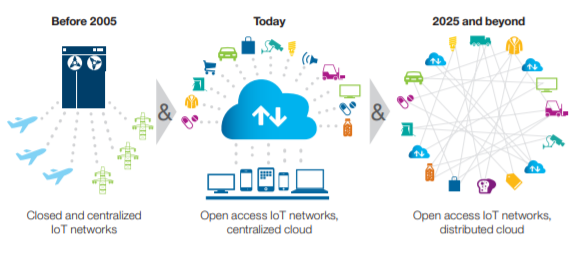
\includegraphics[width=3.5in]{ibm.png}
}
Another benefit of this would be that decentralisation would remove the single point of failure that the centralised model currently has. This is what the figure above made by IBM \cite{ref12} demonstrates. This is because the network wouldn't rely on one server for all operational needs, rather the network would use all the nodes on the blockchain. \cite{ref6} \cite{ref11} This would add a lot of reliability to the IoT which in turn would increase widespread adoption.
\par Decentralisation would enable peer to peer messaging which would save a lot of cost and resources. For example, take the smart traffic light example that was given in the introduction. If the cameras on the traffic lights and the lights themselves were IoT devices that used the client-server model, then they would have to use the server to communicate with each other even though they were right beside each other. However, if they were blockchain enabled devices then they could utilise the blockchain to enable peer to peer messaging. This would allow them to communicate directly with each other which would be much more efficient than the former option.
\par However, while blockchain removes a single point of failure, it could potentially introduce a bottleneck too. The authors of \cite{ref7} say this is likely to happen because a lot of current blockchains can only handle a low amount of transactions per second. For example, Bitcoin (the original blockchain) can only handle 7 transactions per second and Ethereum, (the second most popular blockchain) can only handle about 20 to 40. This number is far too low for the potential hundreds of billions of IoT devices. However, what the authors of this piece don't point out is that there are a number of new blockchains such as Polkadot aiming to solve these issues through a process called sharding. Sharding is a process of running many chains in parallel. \cite{polka}.

\centerline{
    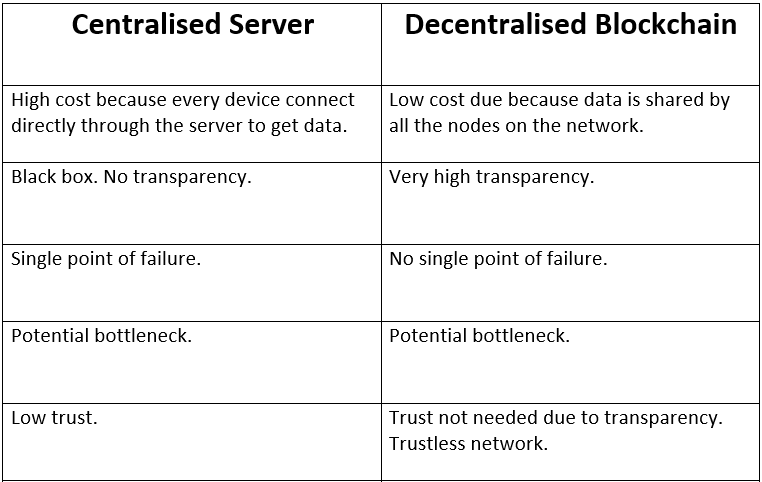
\includegraphics[width=3.5in]{table.png}
}
This table gives a summary of the comparisons made between the centralised and decentralised model in this review. 

\section{Integration Issues}
Most of the literature presented here is very enthusiastic about the integration of blockchain and IoT, and there are clear benefits for doing so. However, there are a couple of glaring issues preventing the integration of the two technologies which are not discussed in the majority of the given sources. One of these is identified by the authors\cite{ref9}. They bring up a point that, currently, a centralised database will outperform a blockchain which relates to the point above about blockchains having low transactional abilities. This is definitely an area that needs more academic attention, but again solutions are being developed by many blockchains in the form of sharding, including Ethereum itself.
\par Another issue, serves as a very big gap in the literature is the question of where to store the proposed blockchain that the IoT devices will use. Blockchain removes the need for a centralised data server by storing the data on each of the nodes on the blockchain. However, currently IoT devices cannot be blockchain nodes due to their low memory capacities. Very few sources analysed in this review bring this up, except for the authors of \cite{where} and \cite{ref6}. While they state that this is a problem, they don't offer any solutions to it. However, the authors of \cite{ref7} propose that IoT devices be lightweight nodes instead of full nodes, meaning that they only store part of the blockchain instead of the full thing. However they also point out that many blockchains do not yet support lightweight nodes. Further research and development in the technology must be done in order to address this issue.

\section{Conclusion}
The main issues with the IoT are security, scalability, data integrity and high cost. These issues all point to a culprit that is the current centralised client-server model. In this review, we discussed the potential benefits to decentralising the IoT by enabling blockchain onto it. The benefits are vast, but it is not without its own drawbacks and challenges. Blockchain enabled IoT has massive potential, but technological advancements have to be made regarding the scalability of blockchains before that potential can come to fruition.

\bibliographystyle{unsrt}
\bibliography{bibliography}

\end{document}
